\section{Reconocimiento de texto en escenas naturales}
	\begin{frame}
		\frametitle{Reconocimiento de texto en escenas naturales}
		Kai Wang, Boris Babenko y Serge Belongie publicaron, en 2011, el paper \textit{End-to-end scene text recognition} en el que se basa este trabajo.
		
		Los autores establecen un conjunto de etapas para el reconocimiento de texto en imágenes naturales. Este trabajo está enfocado específicamente en la etapa de \textbf{reconocimiento de caracteres}.
	\end{frame}
	\subsection{Reconocimiento de caracteres}
		\begin{frame}
			\frametitle{Detección de caracteres}
			\framesubtitle{Algoritmo de ventana deslizante}
			\begin{center}
				
\includegraphics[height=0.65\paperheight]{imgs/ventana_deslizante.png}
			\end{center}
		\end{frame}
		\begin{frame}
			Los sistemas que emplean esquemas de reconocimiento de caracteres usualmente deben funcionar en tiempo real y evaluar una gran cantidad de ventanas.
			\begin{itemize}
				\item<1->[]
				\item<2->[] Se decide usar \textbf{Random Ferns} como clasificador.
					\begin{itemize}
						\item<2-> Es eficiente.
						\item<3-> Puede manejar múltiples clases.
					\end{itemize}
			\end{itemize}
		\end{frame}
		% RANDOM FERNS
		\begin{frame}
			\frametitle{Random Ferns}
			\begin{itemize}
				\item<1-> Es un clasificador probabilístico propuesto por Ozuysal et. al. en 2010.
				\item<2-> Es ``ensemble'', compuesto por un determinado número de entidades o clasificadores.
				\item<3-> Hace uso de descriptores de características binarios.
			\end{itemize}
		\end{frame}
		%%%%%%%%%%%%%
		\begin{frame}
			\frametitle{Extracción de características}
			\framesubtitle{Característica}
			\begin{definition}
				Una característica es una propiedad que distingue a un objeto de otros. Es decir, algo que lo hace único.
			\end{definition}
		\end{frame}
		\begin{frame}
			\frametitle{Extracción de características}
			\begin{itemize}
				\item<1->[] El objetivo es, dada una ventana con un caracter, extraer el vector de características.
				\item<2->[] En la literatura de clasificación y reconocimiento en imágenes naturales, un vector de características muy empleado es \textbf{HOG}.
			\end{itemize}
			\begin{center}
				\includegraphics<1->[height=0.25\paperheight]{imgs/letra_N.png}
			\end{center}
		\end{frame}
		\begin{frame}
			\frametitle{HOG}
			\begin{definition}
			Los histogramas de gradientes orientados (HOG por su sigla en inglés) son descriptores de características que moldean la distribución del grandiente de una imagen y está definido en $\mathbb{R}^N$.
			\end{definition}
		\end{frame}
		\begin{frame}
			\frametitle{HOG}
			Ventajas:
			\begin{itemize}
				\item<1-> Son fáciles de computar.
				\item<2-> Son compactos.
				\item<3-> Se pueden almacenar fácilmente.
				\item<4-> Son fáciles de comparar.
			\end{itemize}
		\end{frame}
		\begin{frame}
			\frametitle{Ejemplo}
			\begin{center}
				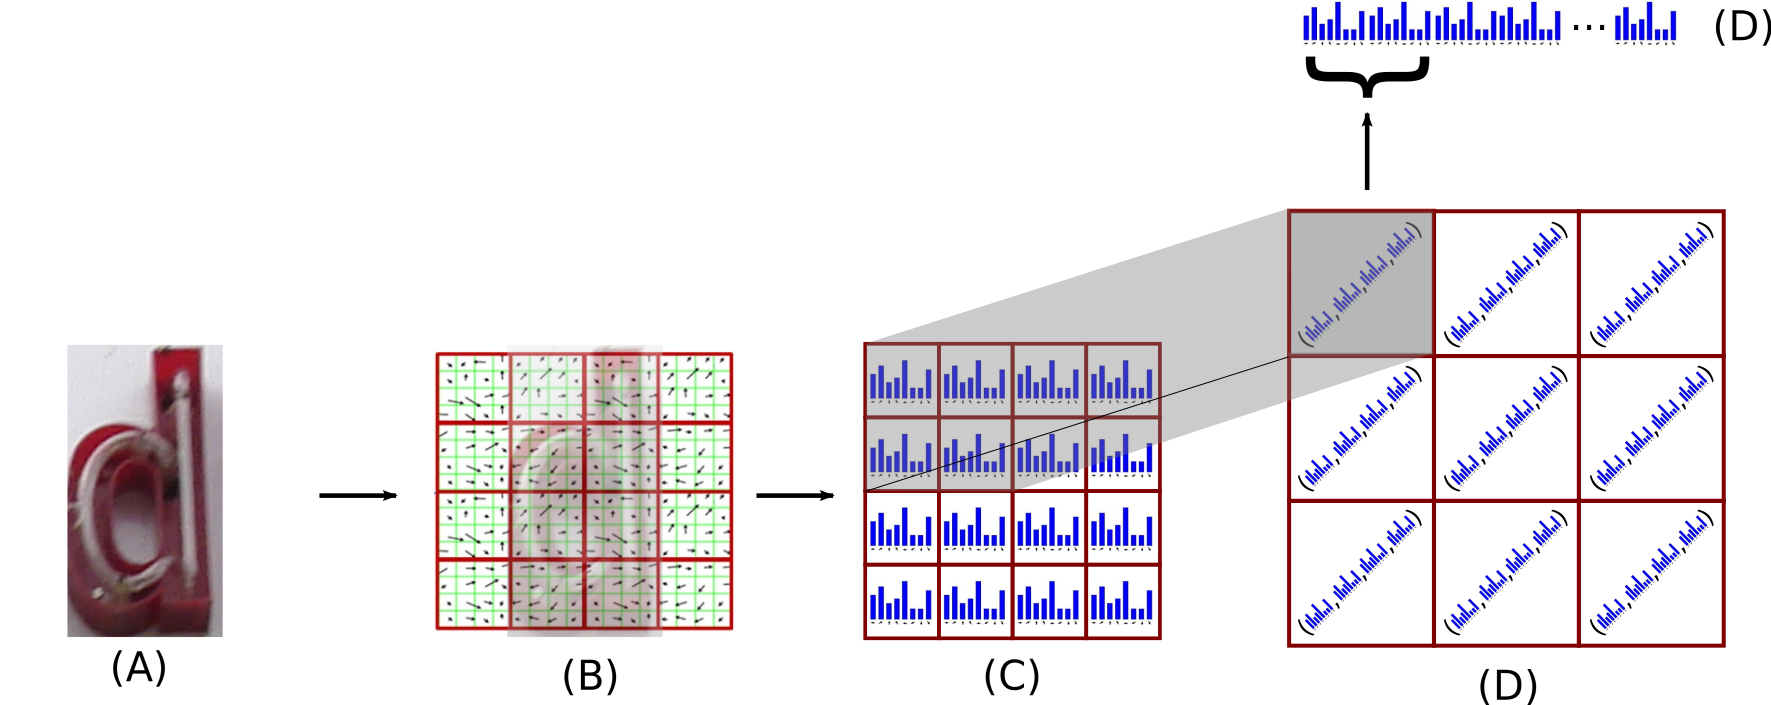
\includegraphics[height=0.45\paperheight]{../img/hog/hog.png}
			\end{center}
		\end{frame}	
		%\begin{frame}
		%	\frametitle{Gradientes}
		%	\begin{center}
		%		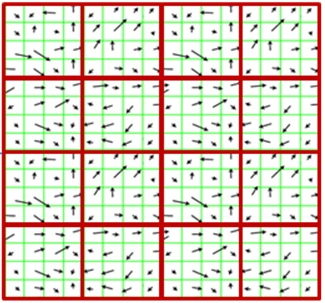
\includegraphics[height=0.45\paperheight]{../img/hog/grid.png}
		%	\end{center}
		%\end{frame}
		\begin{frame}
			\frametitle{Binarización}
			\alert{Warning!}	\textit{Random Ferns necesita de vectores binarizados}.
			
			Para poder utilizar los descriptores \textit{HOG} con \textit{Random Ferns} es necesario establecer esquemas de binarización.
		\end{frame}
		%\begin{frame}
		%	\frametitle{Ejemplo}
		%	\begin{center}
		%		\includegraphics<1>[height=1\paperheight]{imgs/binarizacion_1.png}
		%		\includegraphics<2>[height=0.75\paperheight]{imgs/binarizacion_2.png}				%		\includegraphics<3>[height=0.70\paperheight]{imgs/binarizacion_3.png}		
		%	\end{center}
		%\end{frame}
		\begin{frame}
			\frametitle{Esquemas de binarización}
			\begin{itemize}
				\item<1-> Media
					$$b(C_i) = \frac{\sum_{j=1}^N c_{i_j}}{N} $$
				\item<2-> Mediana
	\[
    		b(C_i) = 
		\begin{cases}
    			\frac{c_{i_{\frac{dim(C)}{2}}} + c_{i_{\frac{dim(C)}{2}+1}}}{2} & \text{si dim(C) es par}\\
    			\frac{c_{i_{\frac{dim(C)}{2}}}}{2} & \text{caso contrario}
		\end{cases}
	\]
				\item<3-> Bootstrap
					$$ b(C_i) = c_{i_k} $$
				\item<4-> Exponencial
					$$\hat{\lambda} = \frac{\sum_{j=1}^N c_{i_j}}{N} $$
			\end{itemize}
		\end{frame}
		%\begin{frame}
		%	\frametitle{Ejemplo (continuación)}
		%	\begin{center}
		%		\includegraphics<1>[height=0.8\paperheight]{imgs/binarizacion_4.png}
		%		\includegraphics<2>[height=0.8\paperheight]{imgs/binarizacion_5.png}				%		\includegraphics<3>[height=0.8\paperheight]{imgs/binarizacion_6.png}
		%		\includegraphics<4>[height=0.8\paperheight]{imgs/binarizacion_7.png}				%		\includegraphics<5>[height=0.8\paperheight]{imgs/binarizacion_8.png}
		%	\end{center}
		%\end{frame}
		\begin{frame}
			\frametitle{Random Ferns (continuación)}
			\framesubtitle{Entrenamiento}
			\begin{center}
				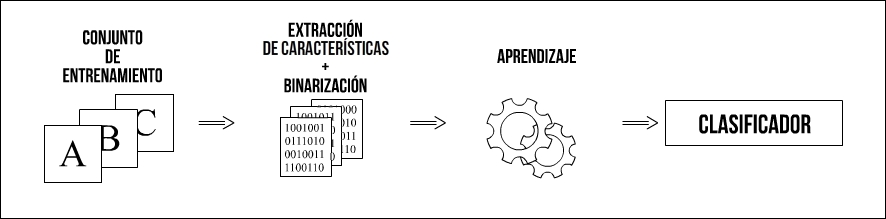
\includegraphics[height=0.30\paperheight]{../img/pipeline_entrenamiento.jpg}
			\end{center}
		\end{frame}
		\begin{frame}
			\frametitle{Random Ferns (continuación)}
			\framesubtitle{Aprendizaje}
			\begin{center}
				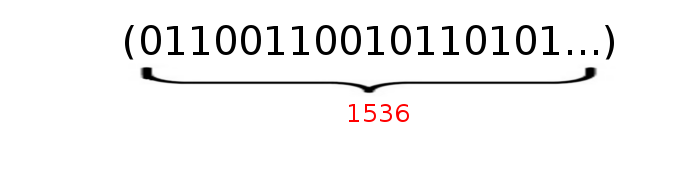
\includegraphics[height=0.30\paperheight]{imgs/aprendizaje_1_1.png}
			\end{center}
			Se necesitaría una tabla con $2^{1536}$ entradas lo cual es computacionalmente imposible de procesar.
		\end{frame}
		\begin{frame}
			\frametitle{Random Ferns (continuación)}
			\framesubtitle{Aprendizaje}
			\begin{itemize}
				\item<1-> Se divide el vector en $M$ grupos o \textit{ferns} de dimensión $S$ y se genera una tabla por cada grupo. Si $M=192 \rightarrow S=8$ entonces:
				\begin{itemize}
					\item<2-> Cada tabla tendría $256$ entradas.
					\item<3-> Se necesitarían $11904$ tablas en total, $192$ por clase.
				\end{itemize}
			\end{itemize}
			\begin{center}
				\includegraphics<1->[height=0.8\paperheight]{imgs/aprendizaje_2.png}		
			\end{center}
		\end{frame}